\cotefile{36}
\scanpage{10}
% Two brown marginal strokes; numeral/letter/bracket interpretation unresolved.
\margin{\handwritten{\figure{\unsure{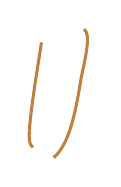
\begin{tikzpicture}[x=0.012cm,y=0.012cm]
\draw[brown,line width=1.1pt] (20,123) .. controls (17,103) and (7,44) .. (7,24) .. controls (7,17) and (8,14) .. (11,12);
\draw[brown,line width=1.1pt] (65,137) .. controls (73,132) and (66,105) .. (62,85) .. controls (56,49) and (50,16) .. (33,1);
\end{tikzpicture}}}}}
\handwritten{\uline{Le théorème de Griffiths par voie algébrique.}}

1.\quad Soit
\[
f:Y\handwritten{\longrightarrow}S
\]
un morphisme propre et lisse de schémas, avec $S$ \inserted{\handwritten{régulier,}} connexe à caractéristiques résiduelles toutes $\ne\unsure{\chi|\ell}$ (nombre premier fixé). Soit $s\handwritten{\in}S$, $\bar s$ un point géométrique au dessus de $s$. Soi\deleted{\unsure{t}}\handwritten{t} $F$ un faisceau $\chi$-adique constant tordu sur $S$ (en pratique, un faisceau de la forme $\underline{Z}_{\chi}(i)$ ), et $x$ une classe de cohomologie
\[
x\handwritten{\in}H^{\deleted{N}\handwritten{\unsure{m}}}(Y,\deleted{\unsure{f(F))|f^*(F))}}\handwritten{F_Y)}\ .
\]
Disons que $x$ est \uline{primitive} si son image dans $H^0(S,R^m f_{\handwritten{*}}\handwritten{(\unsure{f|F}))}\deleted{(F))}$ est nulle, ou ce qui revient au même par le th. de spécialisation de la cohomologie, si son image dans $H^{\deleted{N}\handwritten{m}}(Y_{\bar s},F_{\bar s})$ est nulle. Alors la suite spectrale de Leray pour $f$ nous donne un élément
\[
u(x)\handwritten{\in}{\unsure{E|\mathbb{E}}}_2^{1,\deleted{\unsure{N|N-1|m-1}}\handwritten{m-1}}=H^1(S,R^{\deleted{\unsure{m|N}}\handwritten{m-1}}_{\deleted{\unsure{2|f}}}f_{\deleted{\unsure{f}}\handwritten{*}}(F_{\handwritten{Y}}))\ .
\]
Donnons une propriété fonctorielle générale de cette classe $u(x)$. Pour ceci, soit $Y'$ lisse et propre sur $S$, et
\[
\unsure{Z|\mathbb{Z}|z}\handwritten{\in}H^N(Y\mathbin{\mathrm{x}}_S Y',G),
\]
de sorte que par le formalisme des correspondances cohomologiques, $z$ définit une application
\[
x'\handwritten{\longmapsto}Z(x'): \quad H^{m'}(Y',F')\handwritten{\longrightarrow}H^m(Y,F),
\]
si on suppose $m=m'+N-\handwritten{2}d^{\handwritten{\prime}}\deleted{\unsure{\mathrm{im}(X'/S)|\mathrm{im}(Y'/S)}}$, et qu'on a un accouplement $F'\mathbin{\ooalign{\hfil$\mathrm{x}$\hfil\cr\hfil$\handwritten{\bigcirc}$\hfil\cr}}G\handwritten{\longrightarrow}F(d')$ (NB $d'$ est la dimension relative de $Y'$ sur $S$, supposée constante, et $(d')$ désigne le twist de Tate\deleted{\unsure{de|xx}}; $F'$ et $G$ désignent des faisceaux $\chi$-adiques constants tordus \inserted{\handwritten{sur $S$}} tout comme $F$). Ceci dit, si $x'$ est primitive, alors il en est évidemment de même de $x=Z(x')$, et on aura de plus
\[
u(Z(x'))=Z(u(x'))\ ,
\]
où le deuxième membre s'explicite en notant que $Z$ définit également, par
% archive sheet number: 9
\scanpage{11}
\handwritten{\mspage{2}}
localisation étale sur $S$, un homomorphisme
\[
a'\handwritten{\longmapsto}Z(a'):\quad R^{m'-1}f'_{\handwritten{*}}({\unsure{E|\mathbb{E}|F|\mathbb{F}|C|G}}_{Y'})\handwritten{\longrightarrow}R^{m-1}f_{\handwritten{*}}(F_Y)\ ,
\]
et par suite un homomorphisme (encore noté par $Z$) des $H^1(S,\ )$ pour les drux membres.

Nous allons appliquer ceci au cas où $Y'$ est une courbe relative $C$ sur $S$, $m'=2$, $x'$ est la classe de cohomologie
\[
x'\handwritten{\in}H^{\unsure{2|\handwritten{2}}}(C,\underline{Z}_{\unsure{\chi|\ell}}(1))
\]
défini par un diviseur relatif de la forme $t_1(S)-t_{\unsure{o|0}}(S)$, où $t_1$ et $t_o$ sont deux sections de $C$ sur $S$. Supposant $C$ à fibres géométriques connexes on voit donc que $x'$ est primitif. (NB on pourrait prendre aussi bien n'importe quel diviseur relatif de degré relatif nul.) On prendra pour $Z$ la classe de cohomologie
\[
Z\handwritten{\in}H^{2n}(Y\mathbin{\mathrm{x}}_S C,\underline{Z}_{\chi}(n))
\]
associée à un cycle algébrique sur $Y\mathbin{\mathrm{x}}_S C$ de codimension $n$, qu'on no\deleted{o}tera aussi $Z$. (NB pour que cette classe de cohomologie soit vrai\deleted{\unsure{e}}ment définie en l'état actuel de la Science, il faut faire des hypothèses restricti\deleted{b}ves genre $S$ de type fini sur un corps, ou $S$ excellent de caractéristique \unsure{nulle} ou le dycle $Z$ un cycle ``relatif'' i.e. de codimension $\handwritten{\leqslant}n$ fibre par fibre
Sous ces conditions, $x$ est la classe de cohomologie
\[
x\handwritten{\in}H^{2n}(Y,\underline{Z}_{\chi}(n))
\]
associée au cycle algébrique
\[
z=Z(t_1)-Z(t_o)
\]
sur $Y$. (NB on suppose que les intersections écrites ont un sens, ou qu'on travaille avec des \uline{classes} de cycles de façon qu'elles en aient un, - ce dernier cas supposant (toujours en l'état actuel de la Science) \unsure{què|qué|que}\deleted{\unsure{ax|xx}} $S$ est de type fini sur un corps.
% archive sheet number: 10
\scanpage{12}
\handwritten{\mspage{3}}
Ceci posé, le cycle $Z$ (\unsure{oa|ou} plutôt, sa classe de cohomologie) définit un homomorphisme naturel
\[
Z:\quad R^1g_{\handwritten{*}}(\underline{Z}_{\unsure{\chi|\ell}}(1))\handwritten{\longrightarrow}R^{\unsure{2|a}n-1}f_{\handwritten{*}}(\underline{Z}_{\chi}(n))\ ,\tag*{(*)}
\]
d'où un homomorphisme
\[
Z:\quad H^1(S,R^1g_{\handwritten{*}}(\underline{Z}_{\chi}(1)))\handwritten{\longrightarrow}H^1(S,R^{2n-1}f_{\handwritten{*}}(\underline{Z}_{\chi}(n)))\ ,\tag*{(**)}
\]
et la compatibilité générale énoncée plus haut nous dit que $u(x)=u(c\chi(z))$ n'est autre que l'image de $u(x')$ du premier membre de \deleted{\unsure{(*)x|(*)}} (**). Nous \unsure{aurons|avrons|a\deleted{v}urons} besoin simplement pour la suite de savoir que \uline{si l'homo\deleted{\unsure{morphismo|morphisme}}\unsure{morphisme|morphismo}\deleted{xx}} (*) \uline{est nul} (\uline{ou ce qui revient au même, si l'homomorphisme correspondant sur les fibres géométriques en} $\bar s$ \deleted{est}
\[
H^1(C_{\bar s},\underline{Z}_{\chi}(1))\handwritten{\longrightarrow}H^{2n-1}(Y_{\bar s},\underline{Z}_{\chi}(n))\tag*{(* bis)}
\]
\uline{est nulle}), \uline{alors il en est de même de} $u(x)\handwritten{\in}H^1(S,R^{2n-1}f_{\handwritten{*}}(\underline{Z}_{\chi}(n)))$.

2.\quad Soit
\[
i:Y\handwritten{\longrightarrow}X
\]
un morphisme de schémas pro\unsure{\deleted{jectif}\handwritten{pre}s|\deleted{jectifs}\handwritten{pres}} et lisses sur un corps algébriquement clos $k$, $n$ un entier. On \deleted{suppose} considère l'homomorphisme
\[
i^{\handwritten{*}}:\quad H^{2n-1}(X,\underline{\deleted{Z}\handwritten{Q}}_{\chi}(n))\handwritten{\longrightarrow}H^{2n-1}(Y,\underline{\deleted{Z}\handwritten{Q}}_{\chi}(n))\ ,\tag*{\handwritten{(***)}}
\]
et on suppose:

a)\quad Il existe un homomorphisme en sens inverse $\unsure{vk|v*|v^*}$, dont la restriction à l'image de\deleted{jxx} $i^{\handwritten{*}}$ soit un inverse à droite de $i^{\handwritten{*}}$, et qui soit ``algébrique'' i.e. donné par un cycle algébrique sur $Y\mathbin{\mathrm{x}}X$. (NB Cette hypothèse est un cas particulier des ``conjectures standart'', donc est sans doute touhours vérifiée; elle est vérifiée en tous cas si $i$ est l'i\deleted{\unsure{x}}nclusion d'une section hyperplane dans $X$, lorsque l'opé\deleted{d}ration $\handwritten{\Lambda}$ sur \deleted{\unsure{X est|Xxest}} la cohomologie de $X$ est algébrique, \deleted{ce} \inserted{propriété} qu'on sait vérifier dans de très nombreux cas, par exemple lorsque $X$ se remonte en car. zéro avec sa polarisation.)
% archive sheet number: 11
\scanpage{13}
\handwritten{\mspage{4}}
b)\quad Pour toute courbe algébrique (propre, lisse, connexe) $\unsure{\mathbb{C}|C}$ sur $k$, et tout cycle algébrique $Z$ sur $Y\mathbin{\mathrm{x}}C$ de codimension $n$, l'homomorphisme correspondant
\[
Z:H^1(C)\underline{\deleted{Z}\handwritten{Q}}_{\unsure{\chi|\ell}}(1))\handwritten{\longrightarrow}H^{2n-1}(Y,\underline{Q}_{\chi}(n))
\]
a son image dans celle de $i^{\handwritten{*}}$ de (***). (NB Si on admet le yoga des motifs, justifiable par les``conjectures standard'', cetté\deleted{\unsure{xxxxé|xxxxx}} condition signifie que le \inserted{\handwritten{plus grand}} morceau \deleted{d\unsure{x|u|e}} ``de niveau 1'' du motif \deleted{Coker} ayant comme réalisation $\chi$-adique $\mathrm{Coker}\ i^{\handwritten{*}}$ est nul).
% xxxxé/xxxxx records the visible cancellation cells and the uncertain last
% accented/e-like remnant; it does not recover an earlier lexical word.

\uline{Sous ces conditions}, \uline{pour tout cycle algébrique} $z\handwritten{\in}Z^n(Y)$ \uline{qui est algébriquement équivalent à zéro}, \uline{il existe un cycle} $z'\handwritten{\in}Z^n(X)$ \uline{algébriquement équivalent à zéro}, e\uline{t un} $z''\handwritten{\in}Z^n(Y)$, tels que
\[
z=i^{\handwritten{*}}(z')+z''\tag*{a')}
\]
b')\quad \deleted{\unsure{l'homx|l'hom|Xhomx}} $z''=Z^{\handwritten{''}}(t_1)-Z^{\handwritten{''}}(t_{\unsure{o|0}})$, où $Z''$ est un \inserted{$\underline{Q}$-}cycle \uline{de codimension} $n$ \uline{sur un}\deleted{e courbe} \uline{produit} $\deleted{C\mathrm{x}}\deleted{X}\handwritten{Y}\mathbin{\mathrm{x}}C$, \uline{induisant un homomorphisme} \uuline{nul} \deleted{de} $H^1(C,\underline{\deleted{Z}\handwritten{Q}}_{\chi}(1))\handwritten{\longrightarrow}H^{2n-1}(Y,\underline{Q}_{\chi}(n))$.
% The final x of cancelled l'homx is a visible extra x-out cell, not a
% securely recovered letter of the cancelled abbreviation.

Démonstration immédiate : on écrit $z=Z(t_1)-Z(t_o)$ avec $Z\handwritten{\in}Z^n(Y\mathbin{\mathrm{x}}C)$, ce $Z$ définit un homomorphisme $Z:H^1(C)\handwritten{\longrightarrow}H^{2n-1}(Y)$, \deleted{dont le} qui par hypothèse b) tombe dans $\mathrm{Im}\ i^{\handwritten{*}}$ donc par hypthèse a) est égal au composé $(iv)Z=i(vZ)$, or $vZ:H^1(C)\handwritten{\longrightarrow}H^{2n-1}(X)$ est algébrique puisque $v$ l'est, donc donné par un cycle algébrique $Z'$ sur $X\mathbin{\mathrm{x}}C$, et si on pose $Z''=Z-(i\mathbin{\mathrm{x}}\mathrm{id}_C)^{\handwritten{*}}(Z\handwritten{'} )$, on aura par construction que $Z''$ induit l'homomorphisme nul $H^1(C)\handwritten{\longrightarrow}H^{2n-1}(Y)$. \deleted{D'autre part} Il suffit alors de poser $\unsure{z'|\mathbb{Z}'|Z'}=Z'(t_1)-Z'(t_o)$, $z''=Z''(t_1)-Z''(t_o)$.

3.\quad Mettant ensemble les réflexions de 1) et 2), on trouve ceci. On se donne des schémas propres et lisses $X$ et $Y$ sur $S$ \inserted{\handwritten{\unsure{règulier|régulier}}} connexe, et un $S$-morphisme
\[
i:Y\handwritten{\longrightarrow}X\ .
\]
% archive sheet number: 12
\scanpage{14}
\handwritten{\mspage{5}}
Onnsuppose \inserted{a) et b) vérifiés pour le morphisme $i_{\bar s}:X_{\bar s}\handwritten{\longrightarrow}X_{\bar s}$ induit} \deleted{que le morphisme induit} pour lesfibres en $\bar s$ (point géométrique \deleted{fixé} de $S$\deleted{, qu'on a intérêt à prendre} au dessus da point \uline{générique} de $S$). \deleted{si $S$ est irréductible pour avoir le maximum de chances de \unsure{pouvoir que|pourvoir que} l'hypothèse sérieuse b). Soit $z$ un cycle} \unsure{a|\deleted{a}} \inserted{Soit} $z\handwritten{\in}Z^n(Y)$ tel que le cycle induit sur $Y_{\bar s}$ soit algébriquement équivalent à zéro, et à fortiori cohomologiquement équivalent à zéro. Donc \unsure{d|\deleted{l}d|\deleted{d}l}a classe
\[
u(z)\handwritten{\in}H^1(S,R^{2n-1}f_{\handwritten{*}}(\underline{Z}_{\unsure{\chi|\ell}}(n))
\]
est définie. Ceci posé, je dis que \uline{cette classe est \deleted{une classe de torsion} contenue dans} $i^{\handwritten{*}}(H^{\deleted{\unsure{0}}1}(S,R^{2n-1}\deleted{\unsure{f|g}}\handwritten{g}_{\handwritten{*}}(\unsure{\underline{\deleted{Z}\handwritten{Q}}|\underline{Z}}_{\chi}(n)))$ \uline{modulo une classe de torsion}, du moins si on \deleted{suppose $S$ japonais de dimension 1, ou même} \deleted{\inserted{On applique 2) à $i_{\bar s}$}} \deleted{\inserted{si,}} se permet de remplacer $S$ par un ouvert non vide(restriction \deleted{sans doute}\inserted{probablement} inutile, mais cet énoncé nous suffira pour ce qu'on veut en faire).

Pour le voir, on applique 2) au morphisme $i_{\bar s}$. La courbe $C$ et le cycle $Z''$ peuvent \unsure{d|\deleted{s}d|\deleted{d}s}e définit déjà sur une extension finie $K$ de $k(s)$, Un argument de trace permet de supposer que $K=k(s)$, et \deleted{quitte à prendre l'adhérence du cycle} on peut supposer que $\unsure{\deleted{Z}C|\deleted{C}Z|\mathbb{C}}$ \deleted{et $Z$} est une courbe propre et lisse relative sur $S$ lui-même, et $Z''$ un cycle sur $\unsure{\mathbb{X}|X|Y}\mathbin{\mathrm{x}}_S C$, \deleted{Alors} et que la formule $z=i^{\handwritten{*}}(z')+z''$ est valable sur $\unsure{\deleted{X}Y|\deleted{Y}X|\mathbb{X}}\mathbin{\mathrm{x}}_S C$. Elle implique une décomposition analogue de $u(z)$, qui est la somme de $i^{\handwritten{*}}(u(z'))$ et de $u(z'')$, de sorte qu'il suffit de prouver que $u(z'')$ est nul. Or $u(z'')$ induit par \deleted{d}construction 2) l'homomorphisme nul $H^1(C_{\bar s})\handwritten{\longrightarrow}H^{2n-1}(Y_{\bar s})$. I\unsure{m|\deleted{l}m|\deleted{m}l} résulte donc bien de 1) que $u(z'')$ est nul, cqfd.

4.\quad Soient $X$ un schéma projectif et lisse de dimension $m$\inserted{\handwritten{sur $k$ Alg. clos,}}, prenons un pinceau de Lefschetz, de façon à obtenir une variété éclatée non moins projective et lisse $\overset{\handwritten{\sim}}{X}$ et un morphisme
\[
\overset{\handwritten{\sim}}{f}:\overset{\handwritten{\sim}}{X}\handwritten{\longrightarrow}\deleted{S\mathrm{x}}P^1_k
\]
% The x in the preceding deletion records a visible extra cancellation cell, not a recovered old lexical x.
% The b in fibres has a long thin, partly interrupted extension of its ascender and an irregular retraced bowl. Pen retouch versus surviving type is uncertain; the mark is treated as part of this letter, not as an independent drawing or additional character.
dont les fi\unsure{\handwritten{b}|b}res sont les sections hyp\deleted{é}erplanes du pinceau. Soit $\unsure{B|S|U|\mathbb{S}}$ un ouvert non vide de $P^1_k$ au dessus duquel $\overset{\handwritten{\sim}}{X}$ soit lisse, et soit $\handwritten{\unsure{j|f}}:Y=\overset{\handwritten{\sim}}{X}\handwritten{|}B\handwritten{\longrightarrow\unsure{S}}$.
% archive sheet number: 13
\scanpage{15}
\handwritten{\mspage{6}}
Soit $P^m(X)$ la partie primitive de la cohomologie $H^m(X,\underline{Q}_{\unsure{\chi|\ell}})$, i.e. le noyau du composé
\[
H^m(X)\handwritten{\longrightarrow}H^m(\overset{\handwritten{\sim}}{X})\handwritten{\longrightarrow}H^m(Y)\handwritten{\longrightarrow}H^0(S,R^m f_{\handwritten{*}}(\underline{Q}_{\chi}))\ .
\]
On trouve donc grâce à I) un homomorphisme (dit ``de Griffiths'')
\[
P^m(X)\handwritten{\longrightarrow}H^1(S,R^{m-1}f_{\handwritten{*}}(\underline{Q}_{\chi}))
\]
(en fait, on y pourrait remplacer $S$ par $P^1_k$, mais \deleted{\unsure{nous at|nous et}} peu\unsure{.} importe ici)
D'ailleurs \deleted{\unsure{l'hom|lthom}} on a un homomorphisme d'immersion canonique
% Objects, labels and comma are typed; the three arrows are pen additions.
\diagram{\begin{tikzcd}[ampersand replacement=\&,column sep=small,row sep=small]
Y\handwritten{\arrow[rr]}\arrow[rr,phantom,"i"]\handwritten{\arrow[dr]}\arrow[dr,phantom,"f"']\&\&X_S\handwritten{\arrow[dl]}\arrow[dl,phantom,"g"]\\
\&S\&{,}
\end{tikzcd}}
induisant
\[
i^{\handwritten{*}}:\quad H^1(S,R^{m-1}g_{\handwritten{*}}(\underline{Q}_{\chi}))=H^1(S,H^{m-1}(X,\underline{Q}_{\chi}))\handwritten{\longrightarrow}H^1(S,R^{m-1}f_{\handwritten{*}}(\underline{Q}_{\chi})).
\]
Ceci dit, \uline{l'image inverse par l'homomorphisme de Griffiths plus haut de} $\mathrm{Im}\ i^{\handwritten{*}}$ \uline{est réduite à zéro}.

Ceci se fait par des calculs explicites essentiellement triviaux, compte tenu de la structure cohomologique connue d'une variété éclatée.

5.\quad Mettant ensemble 3) et 4), on trouve ceci:

% The interlinear insertion is typed; a pen guide brings it before "soit".
% The first Y-subscript repeats the s/t-shaped overlap marked at "soit"; later clean s cells do not inherit that overlap. The final x in each of Sousx and the cancelled m=2nx records a visible cancellation cell, not a recovered old lexical letter.
\deleted{Sousx} Avec les notations de 4), \inserted{supposant $m=2n$,} soit $\unsure{s|\deleted{t}s|\deleted{s}t}$ le point générique de $P^1_k$, et \uline{supposons que l'immersion} $Y_{\bar s}\handwritten{\longrightarrow}X\mathbin{\ooalign{\hfil$\mathrm{x}$\hfil\cr\hfil$\unsure{\mathrm{O}|\handwritten{\bigcirc}}$\hfil\cr}}_k k(\bar s)$ \uline{de la section hyperplane} gén\uline{érique} \deleted{dans} s\uline{atisfasse aux conditions} a) e\uline{t} b) d\uline{e} 2).\deleted{(Alors pour On suppose de plus $m=2n$x} \uline{Alors pour tout} $z\handwritten{\in}Z^n(X)$ \uline{dont la restriction à} $Y_{\bar s}$ e\unsure{\uline{s}|s}\uline{t algébriquement équivalent à zér}o, $z$ \uline{est cohomologiquement équiva}le\unsure{\uline{n}|n}\uline{t à zéro} (mod torsion). \deleted{En d'autr} Par suite, le groupe quotient du groupe des cycles cohomologiquement équivalents à zéro \deleted{mod torsion} sur $Y_{\bar s}$, modulo ceux qui sont algébriquement équivalents à zéro (groupe qui mérite le nom de \uline{groupe de Griffiths} $\mathrm{Grif}\unsure{\handwritten{(}|\deleted{t}\handwritten{(}|t}Y_{\bar s})$ de $Y_{\bar s_{\deleted{\unsure{x|k}}}}$),\deleted{contient} tensoris\unsure{é} par $\underline{Q}$, contient comme sous-espace le sous-espace $P^{2n}_{\mathrm{alg}}(X)$ formé des classes de cohomologie primitives sur $X$ qui sont \uline{algébriques}, - vectoriel qui a
% archive sheet number: 14
